% (The MIT License)
%
% Copyright (c) 2023-2024 Yegor Bugayenko
%
% Permission is hereby granted, free of charge, to any person obtaining a copy
% of this software and associated documentation files (the 'Software'), to deal
% in the Software without restriction, including without limitation the rights
% to use, copy, modify, merge, publish, distribute, sublicense, and/or sell
% copies of the Software, and to permit persons to whom the Software is
% furnished to do so, subject to the following conditions:
%
% The above copyright notice and this permission notice shall be included in all
% copies or substantial portions of the Software.
%
% THE SOFTWARE IS PROVIDED 'AS IS', WITHOUT WARRANTY OF ANY KIND, EXPRESS OR
% IMPLIED, INCLUDING BUT NOT LIMITED TO THE WARRANTIES OF MERCHANTABILITY,
% FITNESS FOR A PARTICULAR PURPOSE AND NONINFRINGEMENT. IN NO EVENT SHALL THE
% AUTHORS OR COPYRIGHT HOLDERS BE LIABLE FOR ANY CLAIM, DAMAGES OR OTHER
% LIABILITY, WHETHER IN AN ACTION OF CONTRACT, TORT OR OTHERWISE, ARISING FROM,
% OUT OF OR IN CONNECTION WITH THE SOFTWARE OR THE USE OR OTHER DEALINGS IN THE
% SOFTWARE.

\documentclass{article}
\usepackage{../osbp}
\newcommand*\thetitle{Gaining Popularity}
\begin{document}

\plush{\osbpTitlePage{8}{}}

\pitch{
  \pptBanner{Quick recap of previous lectures:}
  \begin{enumerate}[label=L\arabic*:]
    \setlength\itemsep{0em}
    \item Be nice, say ``Please,'' ``Thanks,'' and ``Sorry''
    \item Expect and enjoy \ul{bug reports}
    \item Make pull requests to others --- boost your \ul{profile}
    \item Prevent chaos by \ul{reviewing} pull request carefully
    \item Make a nice \ul{\texttt{README}} and use \ul{MIT} license
    \item Setup many GitHub Actions \ul{jobs}
    \item Make frequent SemVer \ul{releases}
  \end{enumerate}}

\qte
  [\nospell{Andre Hora}]
  {andre-hora}
  {We found that general models, i.e., models produced using the top GitHub repositories, start to provide \ul{accurate predictions} when they are trained with data from six months and used to predict the number of stars six months ahead.}
  {borges2016predicting}
\pitch{
  \begin{multicols}{2}
  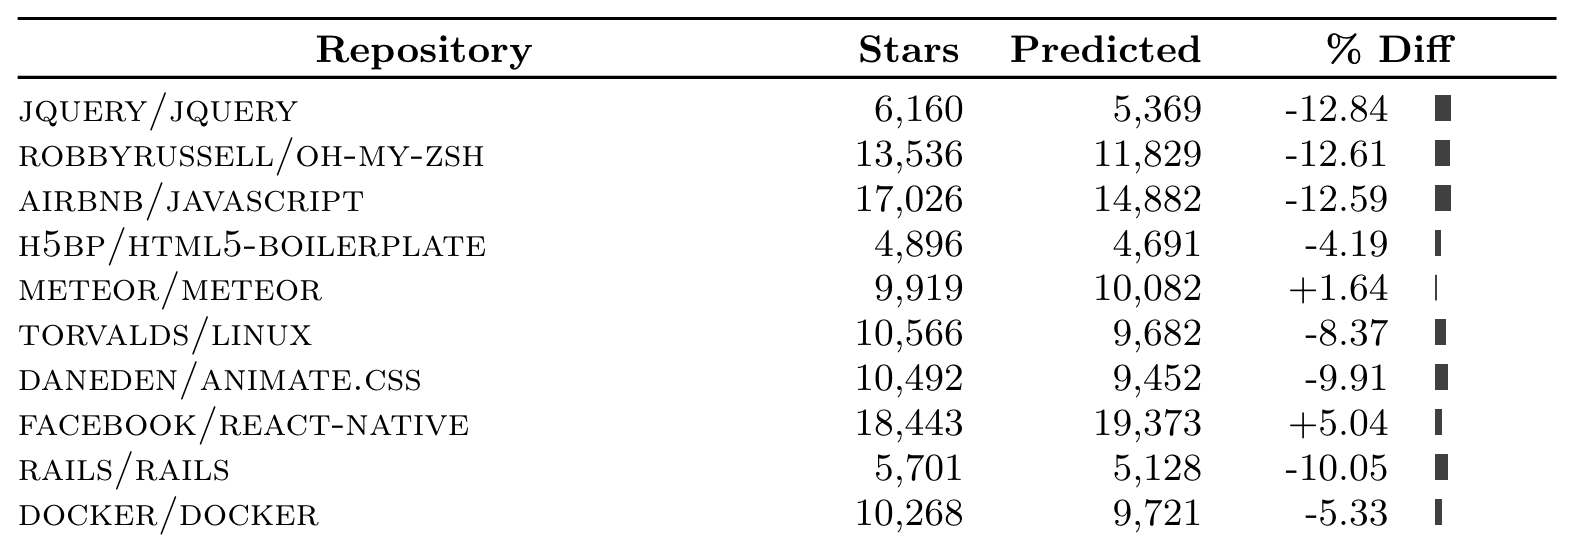
\includegraphics[width=\linewidth]{diff.png}
  \source{borges2016predicting}
  \par\columnbreak\par
  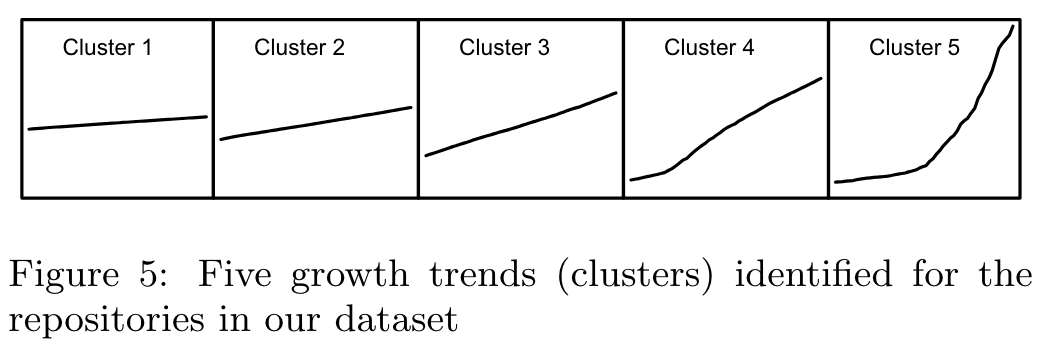
\includegraphics[width=\linewidth]{trends.png}
  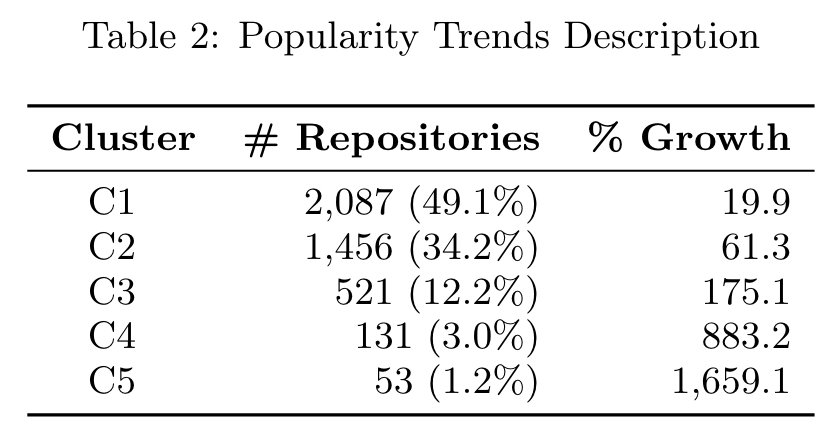
\includegraphics[width=\linewidth]{clusters.png}
  \end{multicols}}

\qte
  [\nospell{Felipe Fronchetti}]
  {felipe-fronchetti}
  {We found that \ul{popularity} of the project (in terms of stars), time to review pull requests, project age, and programming languages are the factors that best explain the newcomers' growth patterns.}
  {fronchetti2019attracts}
% \pitch{
%   \begin{multicols}{2}
%   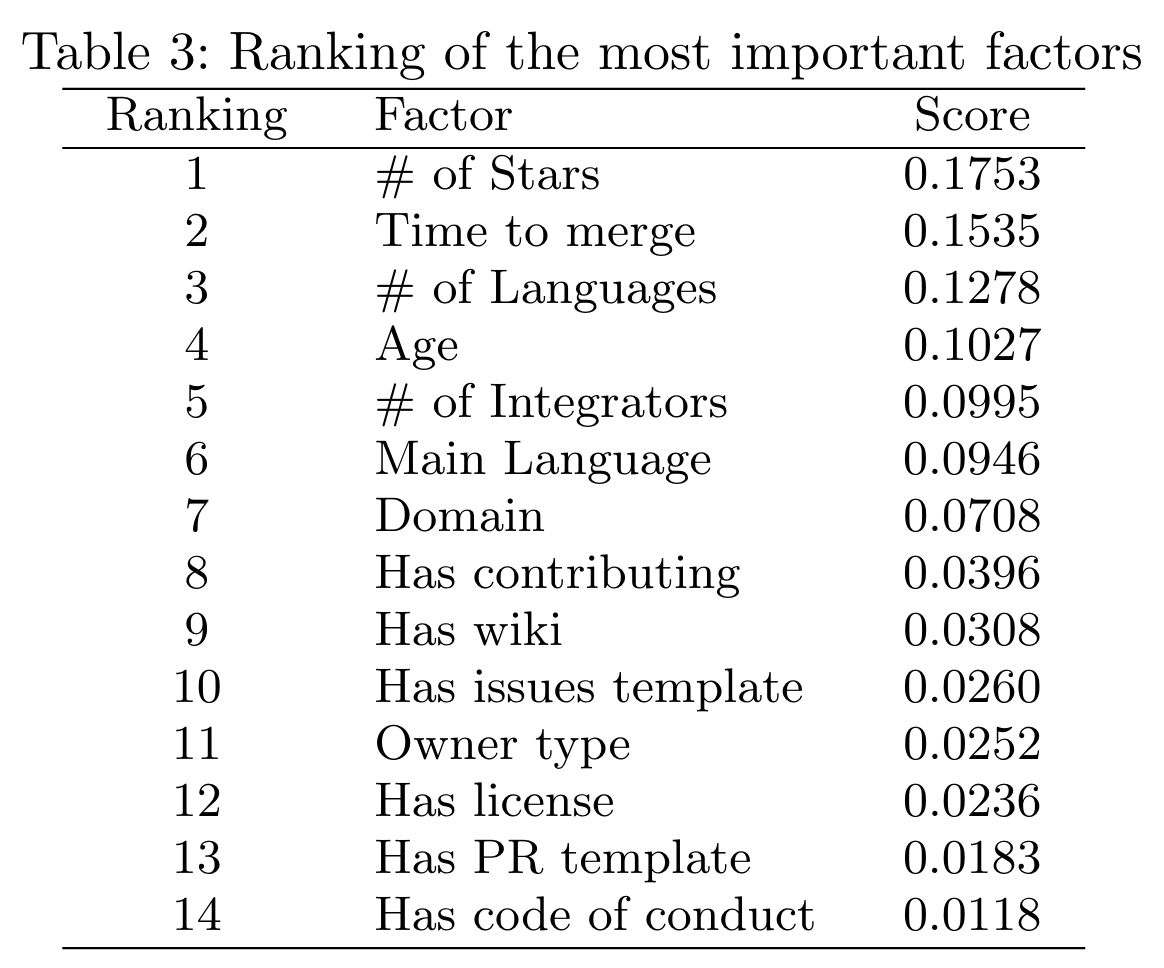
\includegraphics[width=.8\linewidth]{ranking.png}
%   \par\columnbreak\par
%   ``Popularity of the project (in terms of stars), time to review pull requests, and project characteristics like age and programming languages are the factors that best explain the newcomers' growth patterns. In addition, GitHub recommended community standards have a lower influence on the observed growth patterns.''
%   \source{fronchetti2019attracts}
%   \end{multicols}}

\thought{Put some badges.}

\pitch{
  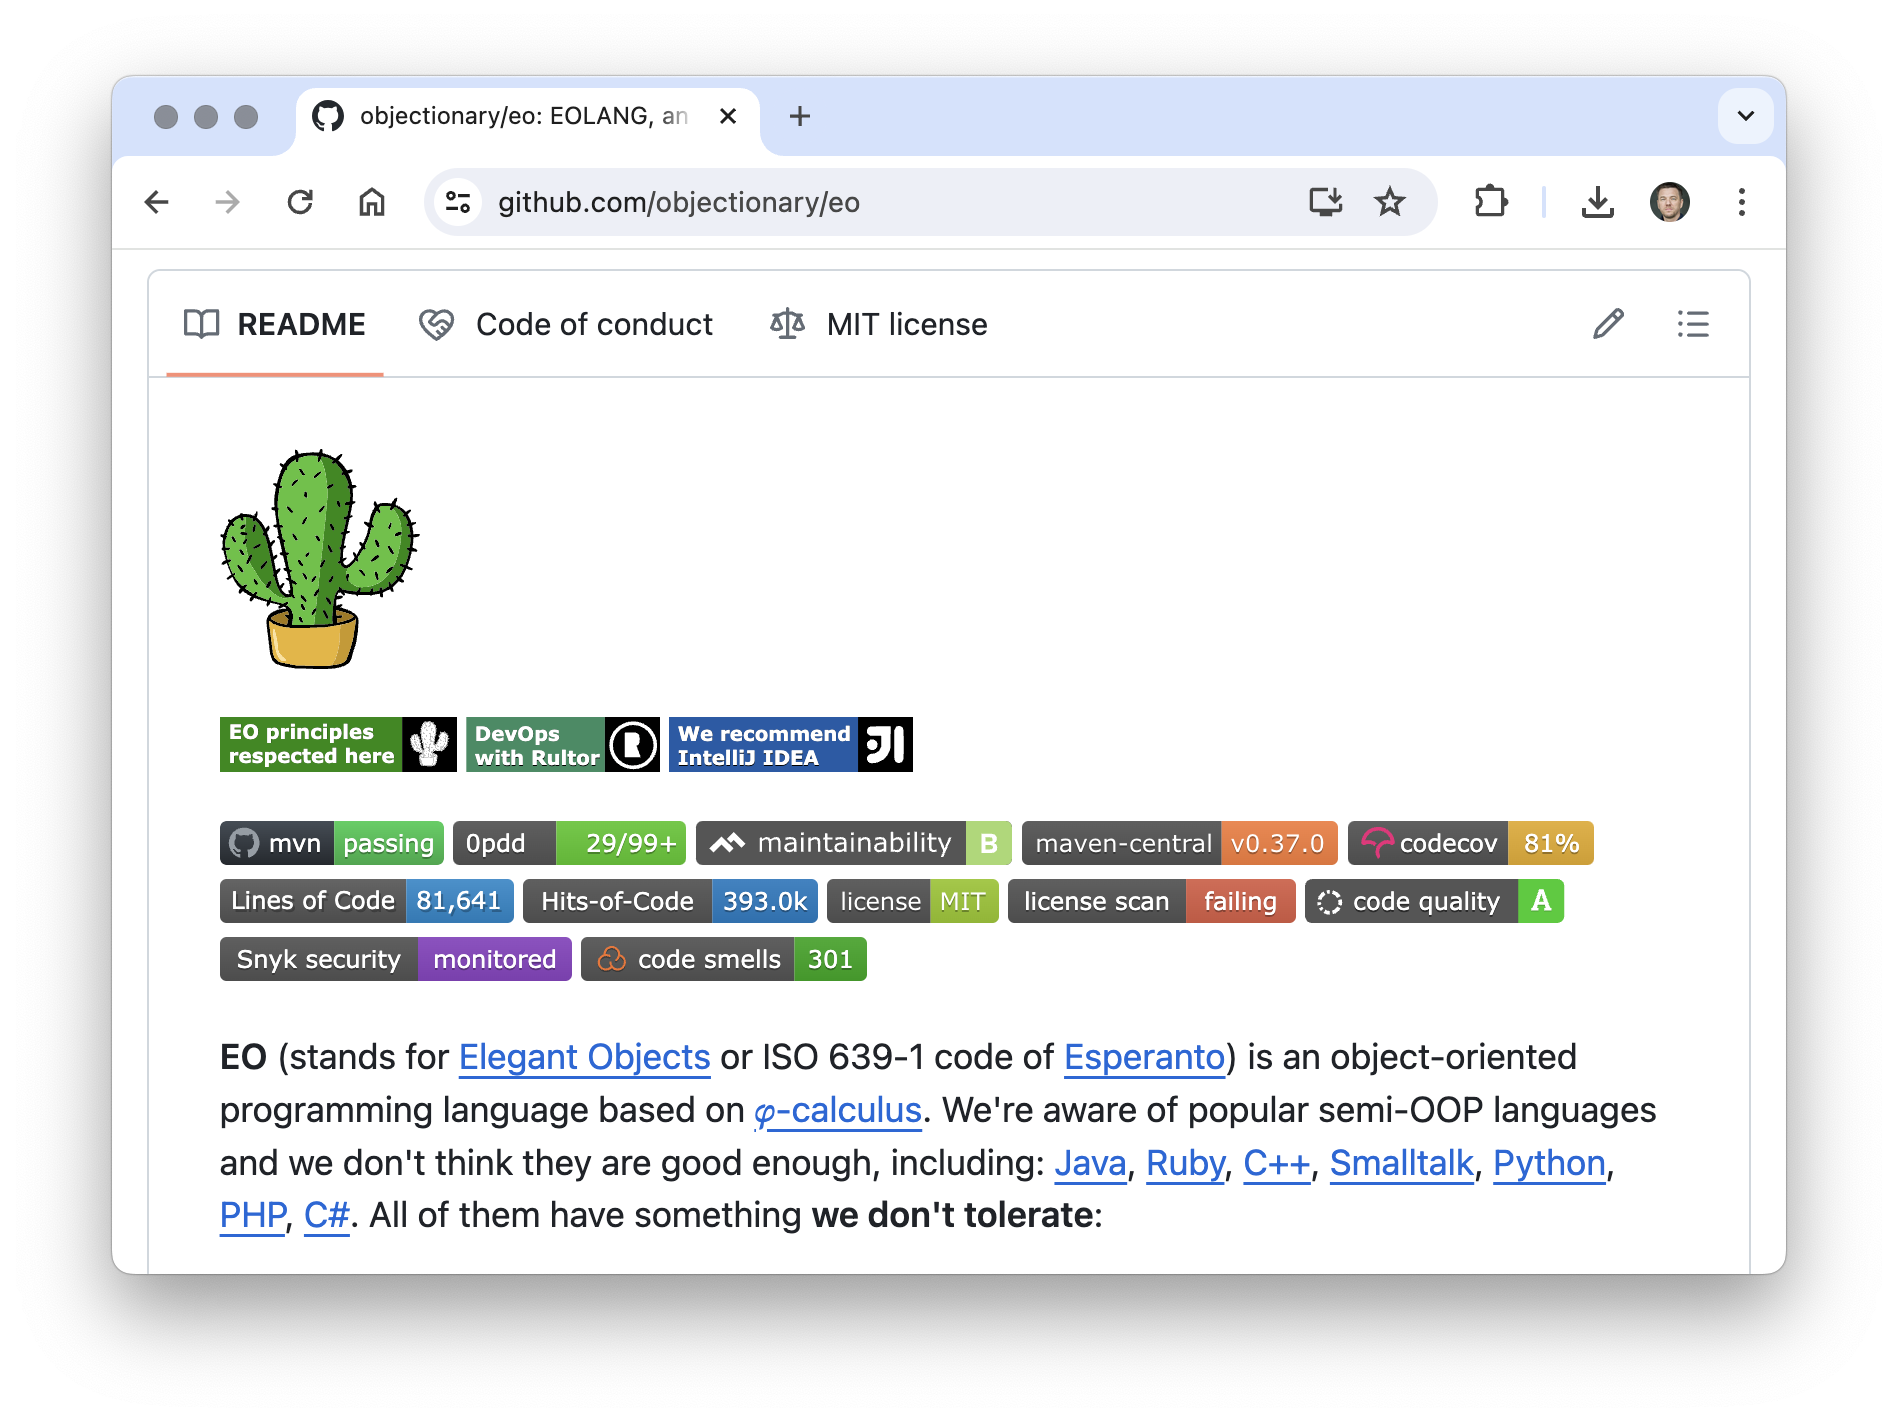
\includegraphics[width=.6\linewidth]{eo-badges.png}
  \par\url{https://github.com/objectionary/eo}}

\qte
  [\nospell{Asher Trockman}]
  {asher-trockman}
  {A vast majority (88\%) agree with the statement `I consider the presence of badges in general to be an indicator of project \ul{quality}.'}
  {trockman2018adding}

\thought{Keep the momentum.}

\qte
  [\nospell{Hudson Borges}]
  {hudson-borges}
  {We concluded that repositories have a tendency to receive more stars right after their \ul{first public release}. After this period, for half of the repositories the growth rate tends to stabilize.}
  {borges2016popularity}

\qte
  [\nospell{Fang Hongbo}]
  {fang-hongbo}
  {We note a sizeable group of people who \ul{follow} others on GitHub and \ul{tweet} about these people’s work, but do not otherwise contribute to those open-source projects.}
  {fang2020need}

\thought{Keep it up.}

\qte
  [\nospell{Tony Ammeter}]
  {tony-ammeter}
  {It appears that \ul{vitality} has a significant effect on popularity over time, indicating that the more active a project is in terms of posting new \ul{releases} and making \ul{announcements}, the more attention it receives from the community.}
  {stewart2002exploratory}

\thought{Make some noise.}

\pitch{
  \pptBanner{Some Places to Announce:}
  \begin{itemize}\setlength\itemsep{0em}
    \item \href{https://www.reddit.com/r/programming/}{Reddit}
    \item \href{https://news.ycombinator.com/}{HackerNews}
    \item \href{https://dzone.com/}{DZone}
    \item \href{https://stackoverflow.com}{StackOverflow}
    \item Telegram Groups
    \item Twitter
    \item Your blog
  \end{itemize}}

\qte
  [\nospell{Marco Tulio Valente}]
  {marco-tulio-valente}
  {We reveal that \ul{Twitter}, \ul{user meetings}, and \ul{blogs} are the most common promotion channels used by the studied projects.}
  {borges2019developers}
\pitch{
  \begin{multicols}{2}
  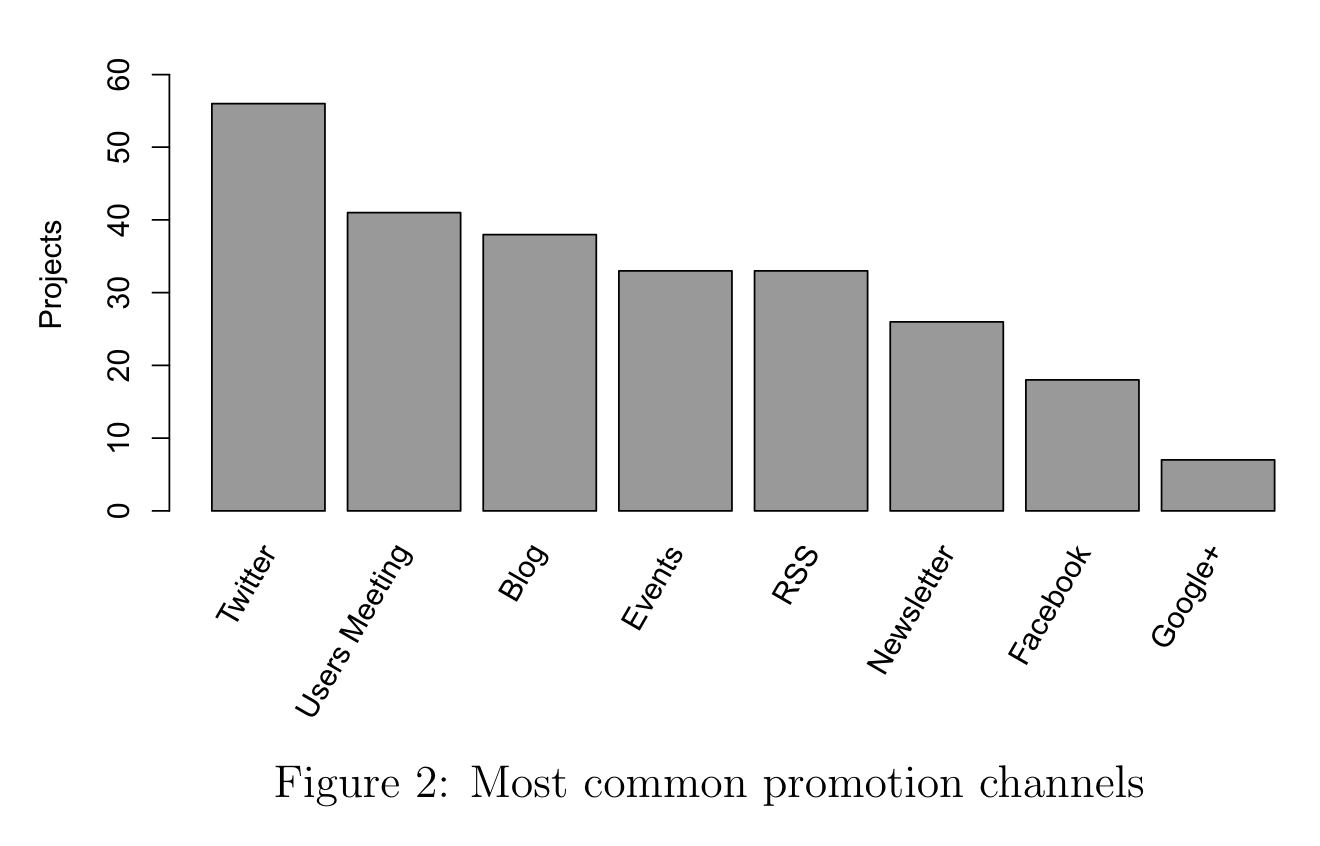
\includegraphics[width=\linewidth]{channels.png}
  \source{borges2019developers}
  \par\columnbreak\par
  The Figure presents the most common promotion channels used by the top-100 projects on GitHub. The most common channel is Twitter, which is used by 56 projects. The second one is Users Meetings (41 projects), followed by Blogs (38 projects), Events (33 projects), and RSS feeds (33 projects).
  \end{multicols}}

\qte
  [\nospell{Hemank Lamba}]
  {hemank-lamba}
  {We find that tweets have a statistically \ul{significant} and practically sizable effect on obtaining \ul{new stars} and a \ul{small} average effect on attracting \ul{new contributors}.}
  {fang2022damn}

\end{document}
